%%%%%%%
% Ch1       %
%%%%%%%

\chapter{Introduction}
	
	\begin{center}
		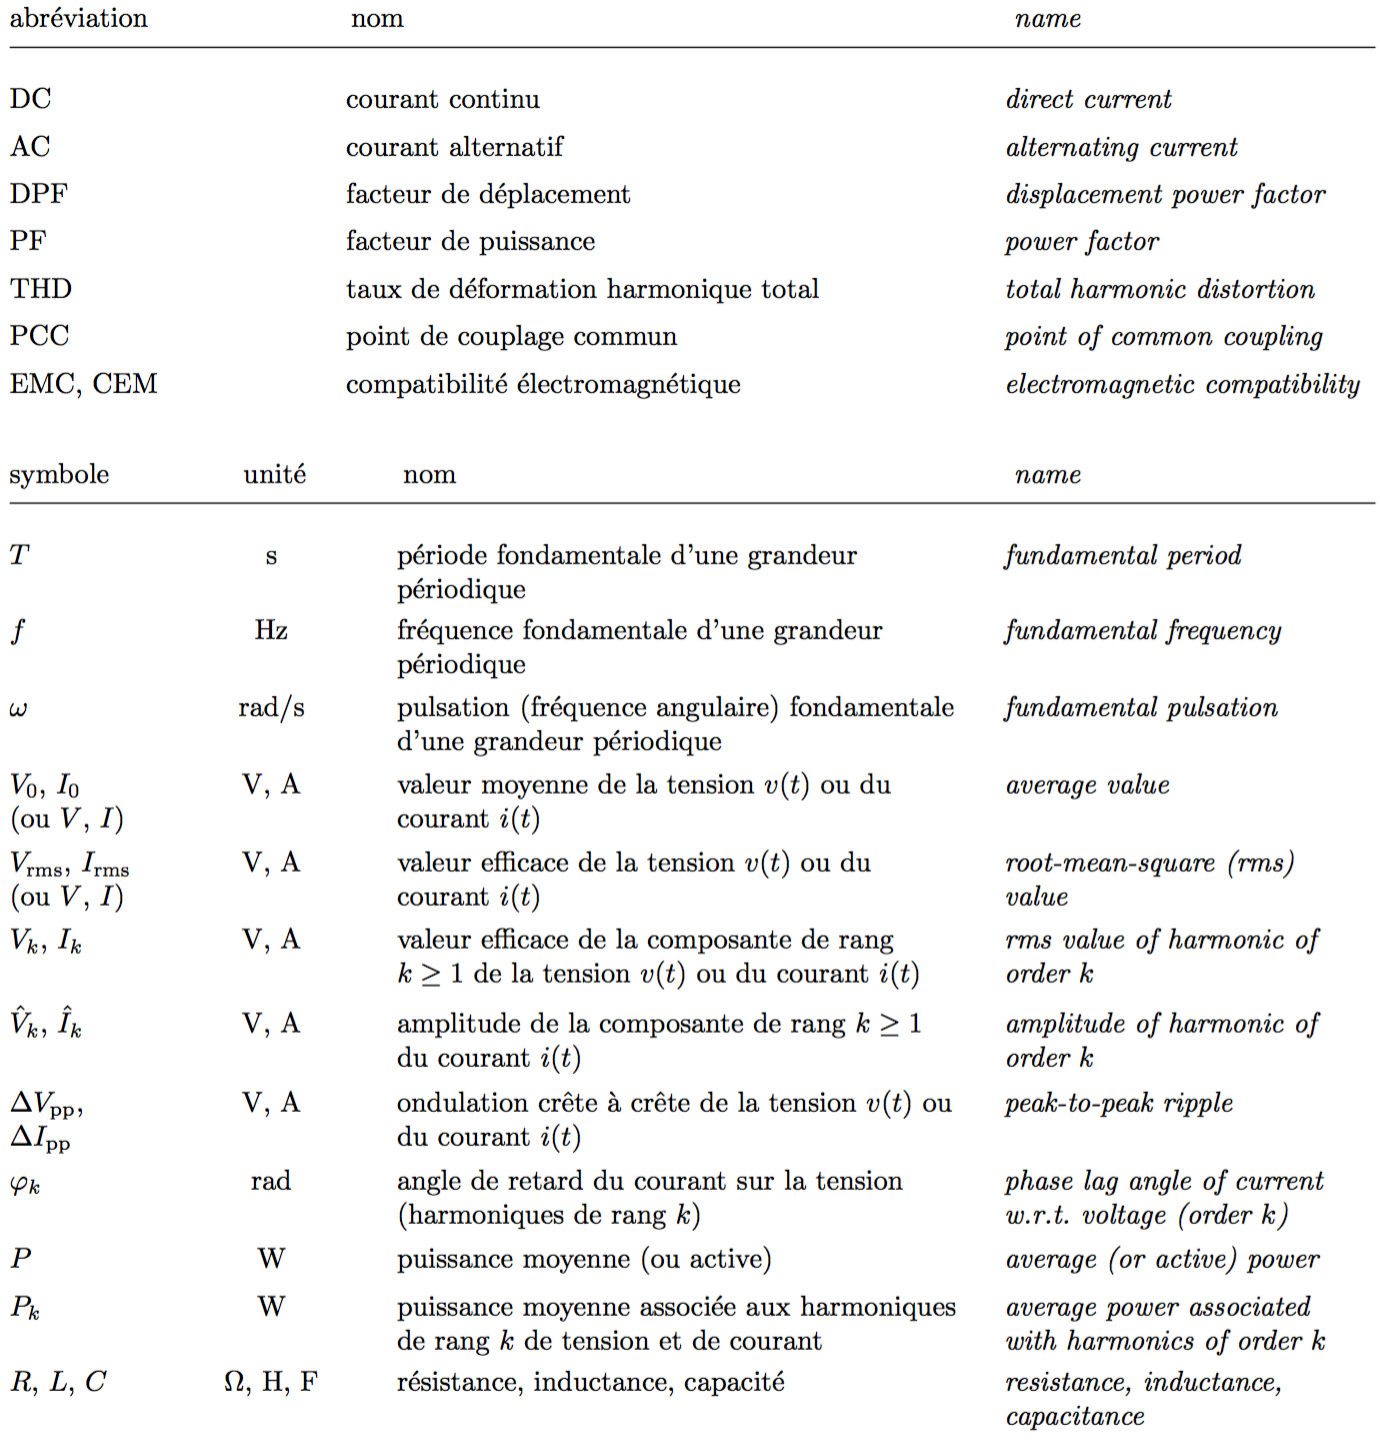
\includegraphics[scale=0.65]{ch1/1}
		\captionof{table}{Liste des abréviations et symboles.}
		\label{table:1.1}
	\end{center}
	
	Ci-dessus se trouve un tableau reprenant les divers abréviations et symboles. 	L'électronique de puissance se distingue de l'électronique de signal par le niveau de puissance élevé. On s'occupe de la conversion de l'énergie d'une forme à une autre et non de la transmission et du traitement des informations analogiques ou digitales. Dans ce cours, on étudiera les convertisseurs quasi tout le temps en fonctionnement en régime établi. La déformation des grandeurs c'est-à-dire leur contenu harmonique est gênante. 
	
\section{Aperçu des différents types de convertisseurs, de composants semi-conducteurs et d'applications}
	\subsection{Types de convertisseurs}
		Les convertisseurs électroniques de puissance effectuent un changement de \textbf{caractéristiques} entre leur entrée et leur sortie. Le \autoref{table:1.2} reprend les principaux. Un convertisseur peut être \textbf{réversible} en puissance, c'est-à-dire que le flux de puissance peut s'écouler aussi bien de l'entrée vers la sortie que vice-versa. Cette propriété est naturelle pour les convertisseurs \textbf{électromagnétiques} (un transformateur par exemple), mais l'est beaucoup moins pour les \textbf{statiques}. Ces derniers contiennent des composants semi-conducteurs qui sont fortement \textbf{non-linéaires}, en plus éventuellement de composants magnétiques et de capacités. 
		
		\begin{center}
			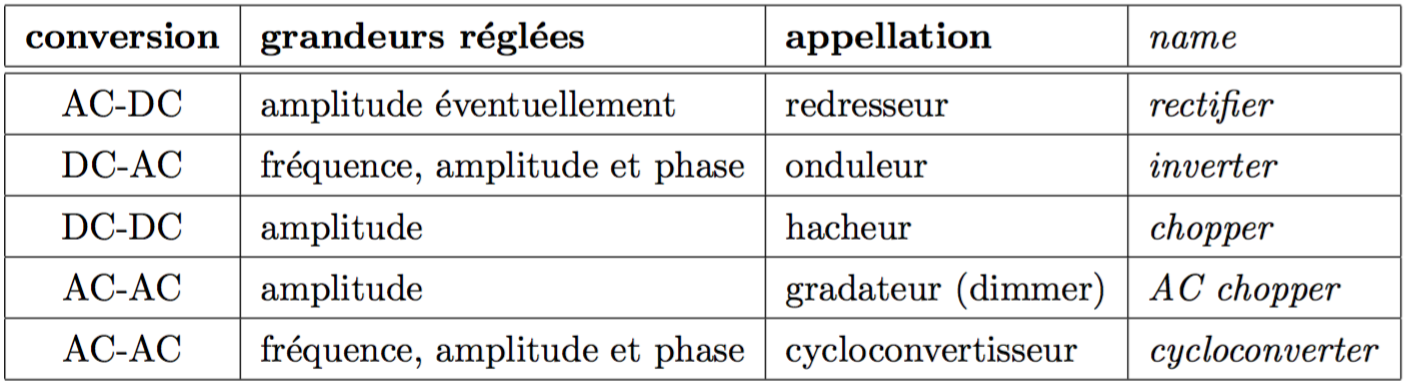
\includegraphics[scale=0.5]{ch1/2}
			\captionof{table}{Types de convertisseurs.}
			\label{table:1.2}
		\end{center}
		
	\subsection{Types de composants semi-conducteurs}
		Les composants semi-conducteurs sont classifiés selon leur commandabilité : 
		
		\begin{itemize}
			\item[•] \textbf{La diode} est un dipôle non linéaire et non commandable. Elle correspond pratiquement à un court-circuit pour un sens du courant et un circuit ouvert pour l'autre. Les \textbf{redresseurs non commandés} constitués de diodes uniquement sont très utilisés. \\
			Capacité en fréquence : faible - grande, en puissance : faible - grande.\\
			
			\item[•] \textbf{Le thyristor} possède en plus de la diode, une électrode de commande qui permet de reporter le début de la conduction, mais pas l'interruption du courant. C'est pourquoi on dit qu'il est \textbf{semi-commandable.}  Avec des \textbf{ponts redresseurs à thyristors}, on peut commander la tension de sortie et en plus l'inverser (dans le cas de l'onduleur). On le retrouve aussi dans les \textbf{gradateurs} et \textbf{cycloconvertisseurs}. Il est \textbf{unidirectionnel} en courant comme la diode. \\
			Capacité en fréquence : faible, en puissance : grande.\\
			
			\item[•] Le \textbf{triac} ressemble au thyristor dans la mesure où il est semi-commandable, mais est \textbf{bidirectionnel} en courant. Cela correspond à la mise en antiparallèle de deux thyristors (tête-bêche). On peut les utiliser dans des \textbf{gradateurs.}\\
			Capacité en fréquence : faible, en puissance : faible.\\
			
			\item[•] La dernière catégorie reprend les composants dont on peut en contrôler aussi bien le début que la fin de la conduction. Il s'agit de \textbf{transistors de puissance} (BJT, IGBT, MOSFET, ...) et de composants dérivés du thyristor (GTO). On parlera d'\textbf{interrupteurs commandables} (switches) qu'on retrouve dans les \textbf{convertisseurs en pont}. On les qualifie d'universels, car on peut faire plusieurs conversions d'énergie (redresseur, onduleur ou hacheur). \\
			Dans l'ordre pour GTO - BJT, IGBT, ... - MOSFET, capacité en fréquence : faible - moyenne - grande, en puissance : grande - moyenne - faible. 
		\end{itemize}
		
	\subsection{Types d'applications}
		\begin{wrapfigure}[9]{l}{3.5cm}
		\vspace{-5mm}
		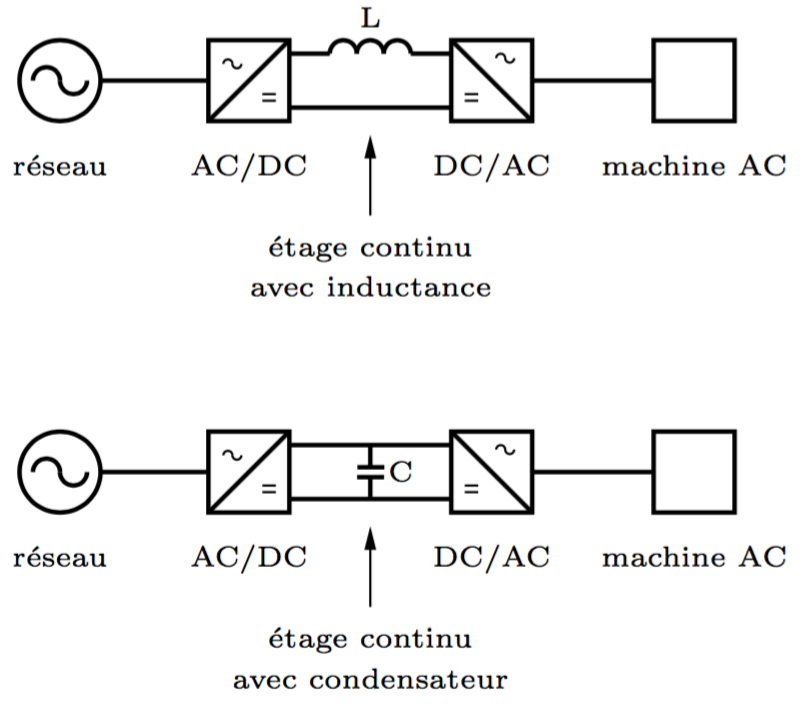
\includegraphics[scale=0.25]{ch1/4}
		\captionof{figure}{}
		\end{wrapfigure}		
		La conversion AC-AC est très utilisée notamment pour l'alimentation et la commande des machines électriques à courant alternatif à partir du réseau. Les gradateurs et cycloconvertisseurs réalisent ceci en une seule étape, mais ont des limitations importantes. On a une plus grande flexibilité avec la mise en cascade d'un convertisseur AC-DC puis DC-AC avec, entre les deux blocs (étage continu commun), soit un condensateur (parallèle) , soit une self (en série) en tant que tampon d'énergie. Le même s'opère pour l'alimentation de machine à courant continu avec un convertisseur AC-DC puis DC-DC. \\
		
		\begin{wrapfigure}[8]{r}{3.5cm}
		\vspace{-5mm}
		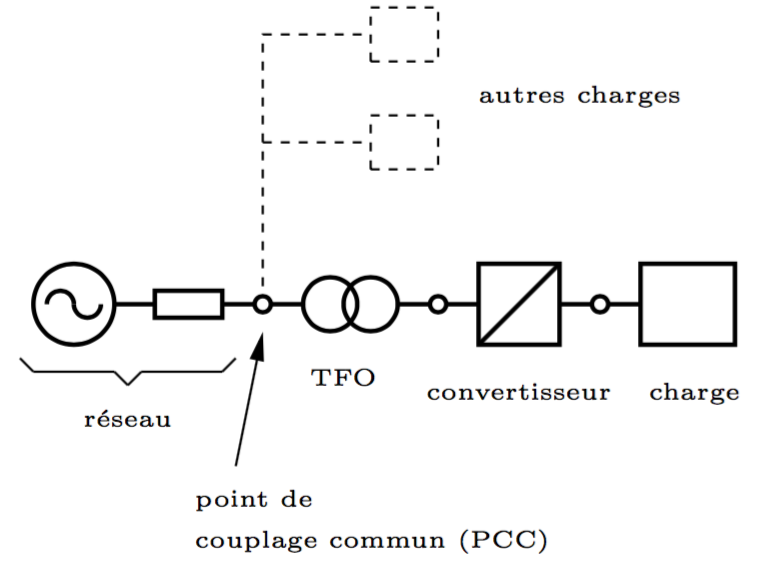
\includegraphics[scale=0.25]{ch1/5}
		\captionof{figure}{}
		\end{wrapfigure}		
		Un convertisseur peut être raccordé au réseau par l'intermédiaire d'un transformateur. En fonction du type de convertisseur et de charge, un courant plus ou moins déformé est tiré du réseau (la charge injecte des harmoniques dans le réseau). Vu l'impédance non nulle du réseau, une tension déformée se présente au niveau du PCC (là où d'autres charges sont raccordées) qui peut conduire à un dysfonctionnement, voire l'endommagement de la charge, auquel cas il y a une \textbf{incompatibilité électromagnétique} (EMC). Le problème des harmoniques peut être réglé par des filtres \textbf{passifs} (inductances et capacités) ou des filtres \textbf{actifs} (convertisseurs avec commande). Pareil entre le convertisseur et la charge pour les déformations. \\
		
		Un autre aspect important est la \textbf{puissance réactive} côté réseau (à tension alternative) et/ou côté charge (à courant alternatif). Certains convertisseurs peuvent fournir de la puissance réactive plutôt que tirer un courant en retard sur la tension. Pour le cas des machines asynchrones à charge par exemple qui consomme de la puissance réactive, ceci est indispensable. La réversibilité du convertisseur niveau puissance active est également importante. Par exemple, le freinage électriquement en récupérant l'énergie ou en la dissipant dans une résistance. 
		
\section{Régimes périodiques et harmoniques}
	\begin{wrapfigure}[6]{l}{5cm}
	\vspace{-5mm}
	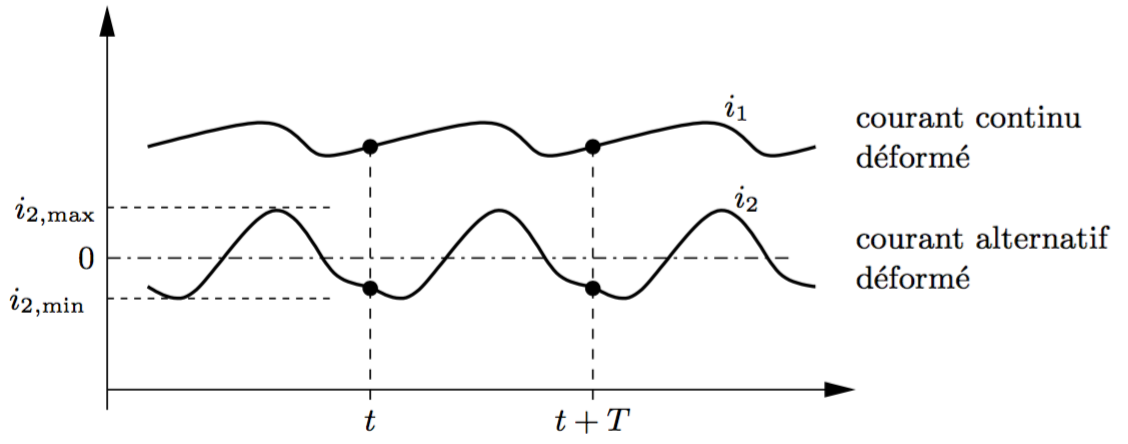
\includegraphics[scale=0.25]{ch1/6}
	\captionof{figure}{}
	\end{wrapfigure}
	On travaillera en régime établi et dans ce cas les courants et tensions possèdent une période fondamentale $T$. Sur la figure ci-contre, le premier signal peut être désigné de continu, car ne change pas de signe et la composante continue est prépondérante alors que le deuxième pas, mais en possède une.
	L'ondulation crête à crête est la différence entre la valeur maximum et la valeur minimum du signal. La fréquence fondamentale $f=1/T$ est directement liée à la fréquence d'alimentation du convertisseur ou à la fréquence de découpage commandée. La présence de composants non linéaires et découpage par interrupteurs déforme les grandeurs : soit non parfaitement constantes, soit non parfaitement sinusoïdales. 
		
	\subsection{Décomposition en série de Fourier}
	Soit un courant périodique $i(t)$ de pulsation fondamentale $\omega = 2\pi f$. Sa décomposition fréquentielle s'écrit : 
	\begin{equation}
	\begin{aligned}
		i(t) &= I_0 + \sum _{k\geq 1} \left(Î_{ck} \cos k\omega t + Î_{sk} \sin \omega t\right)\\
			&= I_0 + \sum _{k\geq 1} \underbrace{Î_k \cos (k\omega t +\gamma _k)}_{i_k(t)} \qquad avec \qquad Î_{ck} - jÎ_{sk} = Î_k e^{j\gamma _k},
	\end{aligned}
	\end{equation}
	où $I_0$ est la composante continue et $i_k(t)$ l'harmonique de rang k. La composante continue donne la valeur moyenne de $i(t)$ sur une période fondamentale puisque les harmoniques sont à valeur moyenne nulle : 
	\begin{equation}
		I_0 = \frac{1}{T}\int _0 ^T i(t)\, dt
	\end{equation}
	Les relations d'orthogonalité à la page 7 du syllabus donnent les relations suivantes pour $k\geq 1$ : 
	\begin{equation}
	\begin{aligned}
		Î_{ck} &= &Î_k \cos \gamma _k &= \frac{2}{T} \int _0 ^T i(t) \cos k\omega t\, dt\\
		Î_{sk} &= &-Î_k \sin \gamma _k &= \frac{2}{T} \int _0 ^T i(t) \sin k\omega t\, dt
	\end{aligned}
	\end{equation}
	
	La \textbf{symétrie demi-onde} (half-wave symetry) se manifeste dans de nombreux cas en pratique, $v(t) = -v(t+T/2)$ ou $i(t) = -i(t+T/2)$. Ceci permet d'annuler les harmoniques de \textbf{rang pair} : 
	\begin{equation}
		\int _0 ^T v(t)\cos k \omega t \, dt = \int _0 ^{T/2} v(t) \underbrace{\left(\cos k\omega t - \cos k\omega(t+T/2)\right)}_{\mbox{= 0 si k est pair}}\, dt
	\end{equation}
	
	\subsection{Valeur efficace}
		La valeur efficace ou rms du courant i(t) est définie comme :
		\begin{equation}
			I_{rms} = \sqrt{\int _0 ^T i^2(t) \, dt} = \sqrt{I_0^2 + \frac{1}{2}\sum _{k\geq 1}Î_k ^2 } = \sqrt{I_0^2 + \sum _{k\geq 1} I_k^2},
		\end{equation}
		où $I_k = \frac{1}{\sqrt{2}}Î_k$ est la valeur rms de l'harmonique de rang $k$. Remarquons que les termes croisés $I_kI_l$ n'apparaissent pas en raison de l'orthogonalité. Considérons un courant parcourant une résistance $R$, les \textbf{pertes Joules instantanés} valent $ri^2(t)$ et celles \textbf{moyennées sur une période fondamentale T} sont données par : 
		\begin{equation}
			P_J = \frac{1}{T}\int _0^T Ri^2 \, dt = RI_0^2 + \sum _{k\geq 1} RI_k^2 = RI_{rms},
		\end{equation}
		et sont donc proportionnelles au carré de la valeur efficace du courant. 
		
	\subsection{Puissances électriques instantanée et moyenne}
		Soit une tension $v(t)$ et un courant $i(t)$ :
		\begin{equation}
			v(t) = V_0 + \sum _{k \geq 1} \underbrace{\sqrt{2} V_k \cos (k\omega t+ \gamma _{vk})}_{v_k(t)} \qquad et \qquad
			i(t) = I_0 + \sum _{k \geq 1} \underbrace{\sqrt{2} I_k \cos (k\omega t+ \gamma _{ik})}_{i_k(t)}
		\end{equation}
		La puissance instantanée dans un système monophasé est donnée par $p(t) = v(t)i(t)$ et celle moyennée 
		\begin{equation}
			P = \frac{1}{T}\int _0 ^T p(t)\, dt = \underbrace{V_0I_0}_{P_0} + \underbrace{V_1I_1\cos \varphi _1}_{P_1} + \sum _{k\geq 2}\underbrace{V_kI_k \cos \varphi _k}_{P_k}
			\label{eq:1.8}
		\end{equation}
		où $P_0$ est la puissance associée aux composantes continues, $P_k$ aux harmoniques de rang $k\geq 1$ et où $\varphi _k = \gamma _{vk} - \gamma _{ik}$ est le retard du courant k sur la tension k. Notons que de nouveau les termes croisés n'apparaissent pas. La sommation dans \eqref{eq:1.8} peut être limité à un seul terme :
		\begin{itemize}
			\item[•] Si la tension $v(t)$ est continue et non déformée ($v(t) = V_0; V_k = 0, k\geq 1$) la puissance moyenne est donnée par $P = V_0I_0$, quelle que soit la déformation du courant. Pareil en inversant tension et courant. 
		 
			\item[•] Si la tension est sinusoïdale non déformée ($v(t) = \sqrt{2}V_1\cos (\omega t + \gamma _v); V_k = 0, k\neq 1$), la puissance moyenne est donnée par $P = V_1I_1\cos \varphi _1$, quelle que soit la déformation du courant. Pareil en inversant tension et courant. 
		\end{itemize}
		Dans les autres cas, les $P_k$ sont souvent négligeable devant $P_0$ ou $P_1$. 
		
	\subsection{Grandeurs continues}
		En l'absence de toute déformation, les grandeurs dites continues sont parfaitement constantes. La déformation du courant $\Delta i(t)$ peut comprendre toutes les harmoniques de rang $k\geq 1$ : 
		\begin{equation}
			i(t) = I_0 + \underbrace{\sum _{k\geq 1} Î_k \cos (k\omega t +\gamma _k)}_{\Delta i(t)}
		\end{equation}
		La valeur efficace de la déformation $\Delta i(t)$ est donnée par : 
		\begin{equation}
			\Delta I_{rms} = \sqrt{\frac{1}{2}\sum _{k\geq 1} Î_k^2} = \sqrt{\sum _{k\geq 1} I_k^2}
		\end{equation}
		Il vient pour la valeur efficace du courant total : 
		\begin{equation}
			I_{rms} = \sqrt{I_0^2+\Delta I^2_{rms}}.
		\end{equation}
		Les pertes Joules supplémentaires dues à la déformation sont données par $R(\Delta I_{rms})^2$. 
		
	\subsection{Grandeurs sinusoïdales (systèmes monophasés)}
		En l'absence de déformation, les grandeurs alternatives sont parfaitement sinusoïdales. L'éventuelle déformation se manifeste en une composante $I_0$ et les harmoniques de rang $k\geq 2$ :
		\begin{equation}
			i(t) = \underbrace{Î_1\cos (\omega t+\gamma _1)}_{i_1(t)} + \underbrace{I_0 + \sum _ {k\geq 2} Î_k \cos (k\omega t + \gamma _k)}_{\Delta i(t)}
		\end{equation}
		La valeur efficace de la déformation est donnée par : 
		\begin{equation}
			\Delta I_{rms} = \sqrt{I_0^2+\frac{1}{2}\sum _{k\geq 2} Î_k^2} = \sqrt{I_0^2+ \sum _{k\geq 2} I_k^2}
		\end{equation}
		Le \textbf{THD - total harmonic distorsion} d'une grandeur AC est défini comme le quotient de la valeur efficace de sa déformation sur la valeur efficace de la composante fondamentale :
		\begin{equation}
			THD = \frac{\Delta I_{rms}}{I_1}
		\end{equation}
		Le \textbf{DPF - displacement power factor} est défini comme le cosinus de l'angle $\varphi _1$, le retard du fondamental de courant sur le fondamental de tension : 
		\begin{equation}
			DPF = \cos \varphi _1.
		\end{equation}
		La \textbf{puissance apparente S} et le \textbf{PF - power factor} sont défini :
		\begin{equation}
			S = V_{rms}I_{rms} \qquad et \qquad PF = \frac{P1}{S} = \frac{V_1I_1\cos \phi _1}{S}
		\end{equation}
		où $P_1$ est la puissance moyenne ou active associée aux fondamentaux. Le PF est souvent inférieur à 1 en raison du déphasage $\varphi _1$ ou encore à la déformation de la tension ou du courant ($V_{rms}>V_1$ ou $I_{rms}>I_1$). Pour la transmission d'énergie AC électrique, une charge est dite idéale si connecté à une source de tension parfaitement sinusoïdale, le courant absorbé l'est de même et est en phase avec la tension. Le DPF et PF valent alors 1. Dans ce cas, la valeur efficace du courant et les pertes Joules sont minimales. 
		
		\subsubsection{Ondes carrée et triangulaire}
			\begin{center}
			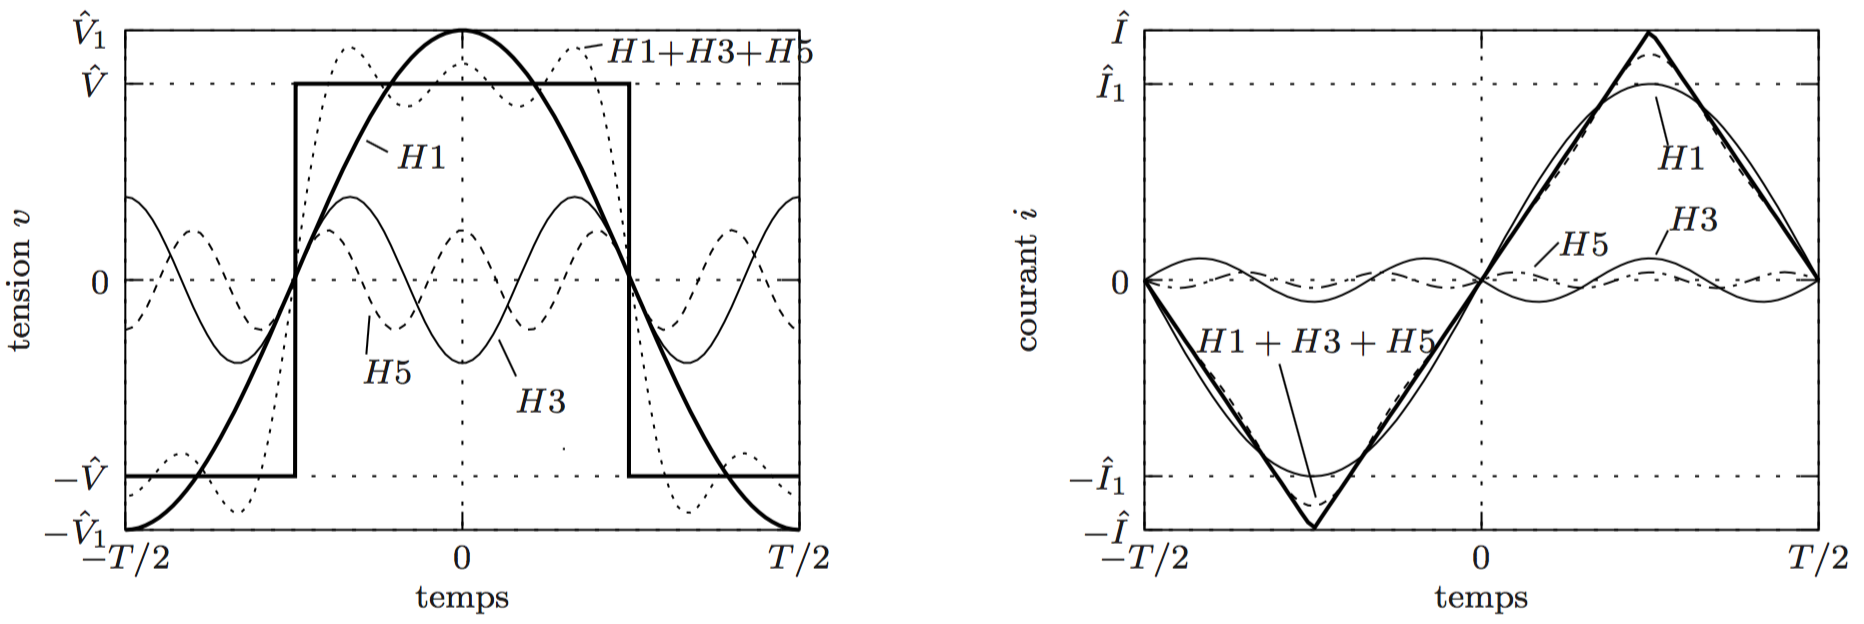
\includegraphics[scale=0.4]{ch1/7}
			\captionof{figure}{}
			\end{center}
			D'après la figure ci-dessus, l'onde carrée de tension varie entre $\hat{V}$ et $-\hat{V}$ et l'amplitude et valeur efficace de la fondamentale sont 
			\begin{equation}
				\hat{V}_1 = \frac{4}{\pi}\hat{V} \qquad et \qquad V_1 = \frac{2\sqrt{2}}{\pi} \hat{V}
			\end{equation}
		   	Les harmoniques de rang pairs étant nulles grâce à la symétrie demi-onde et l'amplitude des harmoniques de rangs $k\geq 1$ étant inversement proportionnelle à leur rang $\hat{V}_k = \frac{1}{k}\hat{V}_1$ : 
		   	\begin{equation}
		   		THD = \sqrt{1/3^2 + 1/5^2+1/7^2+ \dots} = 48.3\%
		   	\end{equation}
		   	Pour l'\textbf{onde triangulaire}, on applique une tension carrée $v(t) = \pm \hat{V}$ sur une inductance L. On a alors un courant triangulaire de pente $\frac{di}{dt}= \pm \frac{1}{L}\hat{V}$. La symétrie demi-onde est de nouveau là et les harmoniques (rang impair) de tension et courant sont lié comme :
		   	\begin{equation}
		   		\hat{V}_k \cos (k\omega t+ \gamma _k) = L\frac{d}{dt}\left( Î_k \sin (k\omega t+ \gamma _k)\right)\qquad \Rightarrow  \hat{V}_k = k\omega L Î_k
			\end{equation}		   	 
			Alors, l'amplitude des harmoniques impaires $k\geq 1$ est $Î_k = \frac{1}{k^2}Î_1$. Le courant est moins déformé que la tension :
			\begin{equation}
				THD = \sqrt{1/3^4+1/5^4+1/7^4+\dots} = 12.12\%
			\end{equation}
		   	De façon dual, un courant carré dans une capacité donnera une tension triangulaire de pente $\frac{dv}{dt} = \pm \frac{1}{C}Î$ et les harmoniques seront liées par : 
		   	\begin{equation}
		   		Î_k = k\omega C \hat{V}_k.
		   	\end{equation}
		   	
	\subsection{Systèmes triphasés symétriques}
		\subsubsection{Régime périodique quelconque}
			Considérons un système de trois courants $i_a(t), i_b(t)$ et $i_c(t)$, de même fréquence et période fondamentale. On parlera de \textbf{symétrique triphasé} lorsque les grandeurs de phase sont décalées de $\pm T/3$, ce qui donne en ordre de phase \textbf{direct} et \textbf{inverse} :
			\begin{equation}
				i_a(t) = i_a(t+T/3) = i_a(t-T/3) \qquad et \qquad i_a(t) = i_a(t-T/3) = i_a(t+T/3)
			\end{equation}
			On parle de \textbf{courants homopolaires} lorsque les 3 courants sont identiques. Pour ce qui est du \textbf{contenu harmonique} dans le cas d'une symétrie d'ordre direct, on suppose la symétrie demi-onde donc pas de rang pair. Le rang $k$ des harmoniques impaires restantes peut être exprimé comme $k = 6m+1, k = 6m +3, k= 6m+5$ (n entier). Les courants se développent comme : 
			\begin{equation}
				i_a(t) = \sum _{k = 6m+1}Î_{a,k} \cos (k\omega t + \gamma _{a,k})+ \sum _{6m+3}Î_{a,k} \cos (k\omega t + \gamma _{a,k}) + \sum _{6m+5}Î_{a,k} \cos (k\omega t + \gamma _{a,k})
			\end{equation}
			La symétrie est aussi d'application au niveau des harmoniques, donc l'amplitude du courant est la même dans les 3 phases. Pour trouver le lien entre les angles de phase, on sait d'après l'ordre des phases direct que :
			\begin{equation}
				\cos (\omega t + \gamma _{a,k}) = \cos (\omega t + \gamma _{b,k} + \frac{2\pi}{3}) = \cos (\omega t + \gamma _{c,k} - \frac{2\pi}{3}). 
			\end{equation}
			\begin{itemize}
				\item[•] $k = 6m+1 :$\\
				On a $\gamma _{a,k} = \gamma _{b,k} + \frac{2\pi}{3} = \gamma _{c,k} - \frac{2\pi}{3}$. Les harmoniques constituent donc un système triphasé d'ordre direct de période $T/k$. 
				\item[•] $ k = 6m+3 :$\\
				On a $\gamma _{a,k} = \gamma _{b,k} = \gamma _{c,k}$, traduisant des systèmes homopolaires lorsque $k = 3, 9, ...$ Lorsque la somme des phases est nulle à tout instant, $i_{a,k}(t)+i_{b,k}(t)+i_{c,k}(t)$. Les harmoniques multiples de 3 sont donc d'office exclus. 
				\item[•] $k = 6m+5$\\
				 On a $\gamma _{a,k} = \gamma _{b,k} -\frac{2\pi}{3} =\gamma _{c,k}+\frac{2\pi}{3}$. Les harmoniques constituent des systèmes triphasés d'ordre inverse. 
				 \newpage
			\end{itemize}
			
		\subsubsection{Onde carrée triphasée}
			\begin{wrapfigure}[10]{l}{4cm}
			\vspace{-5mm}
			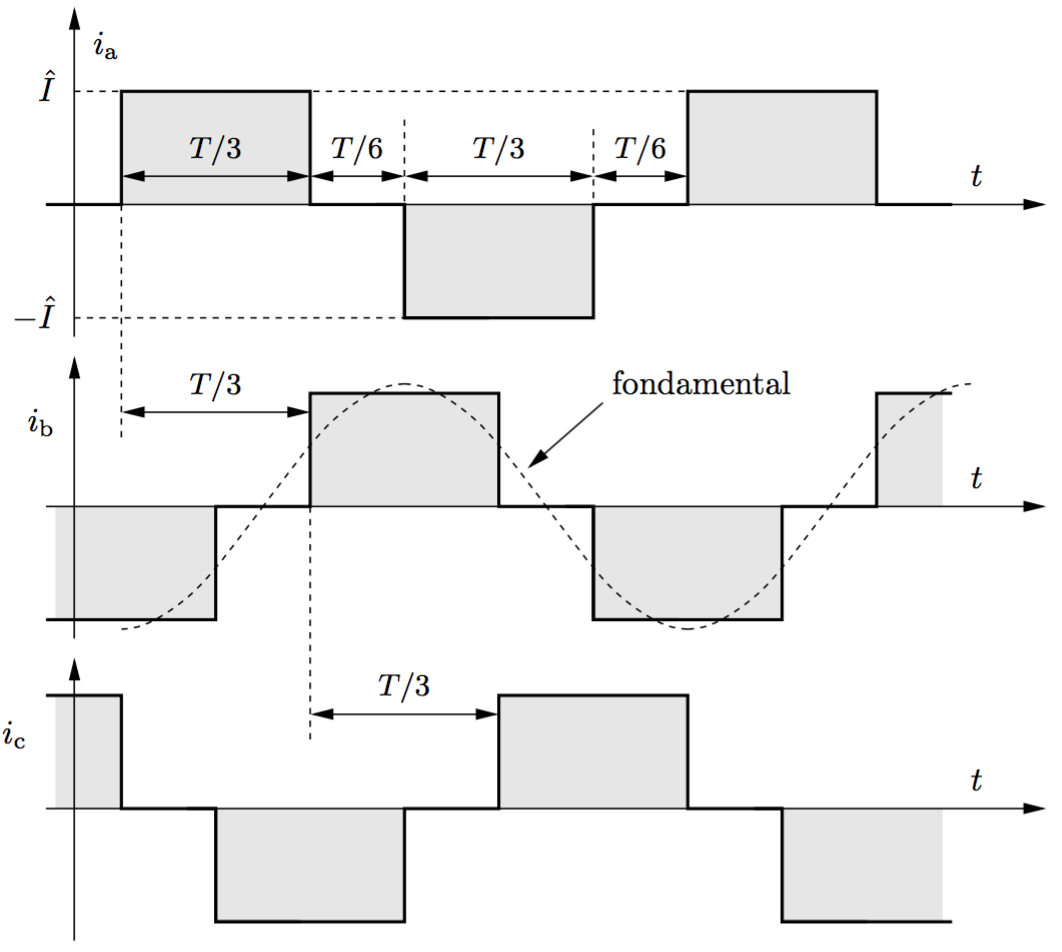
\includegraphics[scale=0.20]{ch1/8}
			\captionof{figure}{}
			\end{wrapfigure}		
			Sur le schéma on voit bien la symétrie d'ordre direct des courants de période fondamentale $T$. Les impulsions positives et négatives de période $T/3$ sont séparées par des intervalles de valeur nulle et de largeur T/6. L'amplitude et la valeur efficace du courant sont donné par 
			\begin{equation}
				Î_{1} = \frac{2\sqrt{3}}{\pi} Î \qquad et \qquad I_1 = \frac{\sqrt{6}}{\pi} Î.
			\end{equation}
			Les harmoniques présentes sont de rang impaire (symétrie demi-onde) et non multiple de 3 (somme des courants nulle). Comme pour le monophasé, on a $Î _k = Î_1/k$ et donc :
			\begin{equation}
				THD = \sqrt{1/5^2 + 1/7^2 + 1/11^2 / \dots} = 31.1\%
			\end{equation}
			
	\subsection{Tension moyenne à travers une inductance et courant moyen à dans un condensateur}
		\subsubsection{Inductance}
			En cas de régime établi de période T, la tension moyenne $v_{L,0}$ est nulle (L cst) :
			\begin{equation}
				v_{L,0} = \frac{1}{T}\int _{t_0}^{t_0+T} v_L (t)\, dt = \frac{L}{T}\int _{t_0}^{t_0+T} \frac{di_L}{dt}\, dt = \frac{L}{T}\left(i_L(t_0 + T) - i_L(t_0)\right) = 0
			\end{equation}
			Aussi dans le cas d'une inductance non linéaire, car le flux périodique $\phi _L(T+t_0) = \phi _L (t_0)$ et $v_L = \frac{d\phi _L}{dt}$. En régime établi, l'inductance absorbe et débite de l'énergie magnétique alternativement selon $e_L(t) = \frac{1}{2} Li_L^2$. Le courant oscille autour de sa valeur moyenne $I_{L,0}$ et l'énergie autour de $E_{L,0}=\frac{1}{2} L I_{L,rms}^2$ à 2 fois la fréquence fondamentale. 
			
		\subsubsection{Condensateur}
			En cas de régime établi de période T, le courant moyen est nul (C cst) : 
			\begin{equation}
				I_{C,0} = \frac{C}{T}\int _{t_0}^{t_0+T} \frac{dv_C}{dt} \, dt = \frac{C}{T} (v_{C}(t_0+T)-v_C(t_0)) = 0
			\end{equation}
			L'énergie électrique accumulé entre les électrodes du condensateur est $e_C(t) = \frac{1}{2}Cv^2_C$. Il débite et absorbe alternativement de la puissance où la tension oscille autour de $v_{C,0}$ et l'énergie autour de $E_C = \frac{1}{2} C V_{C,rms}^2$.
